\subsubsection{Diagrammi di sequenza}
Di seguito il diagramma di sequenza del modulo \textbf{Back-end\ped{G}} realtivo a:
\begin{itemize}
	\item Ricezione prodotto (Figura \ref{fig:getProduct});
	\item Creazione prodotto (Figura \ref{fig:createProduct}).
\end{itemize}

\vspace{1cm}

\begin{figure}[H]
\centering
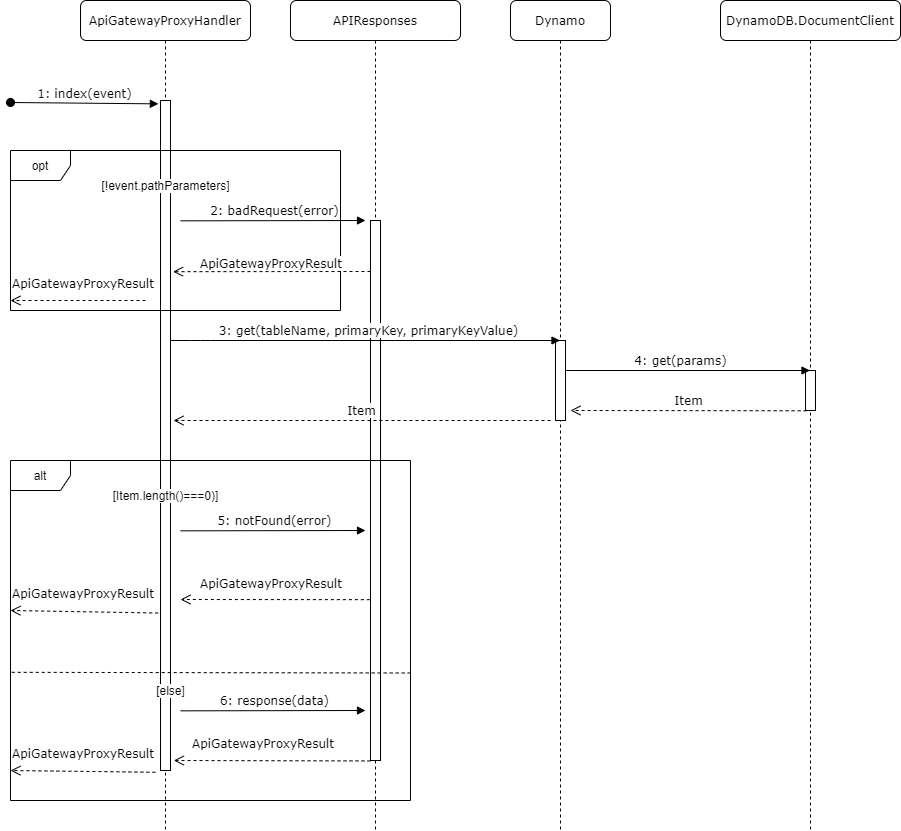
\includegraphics[scale=0.43]{res/Architettura/Backend/img/diagrammaSequenzaRicezioneProdotto.png}\\
\caption{Diagramma di sequenza della ricezione di un prodotto del modulo Back-end\ped{G}}
\label{fig:getProduct}
\end{figure}

\vspace{1cm}

\begin{figure}[H]
\centering
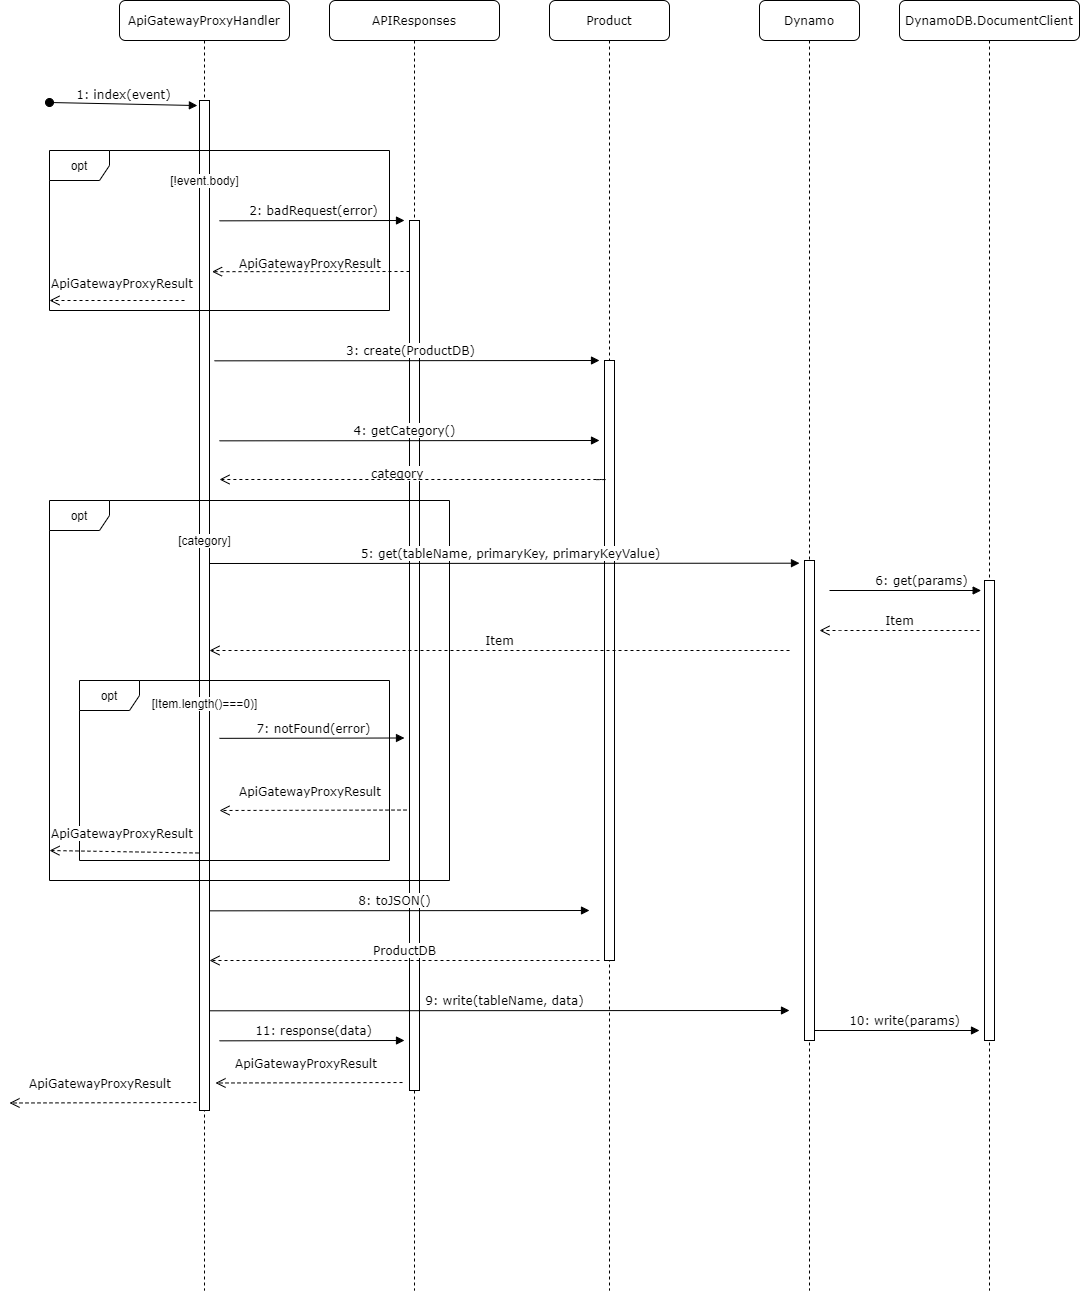
\includegraphics[scale=0.40]{res/Architettura/Backend/img/diagrammaSequenzaCreazioneProdotto.png}\\
\caption{Diagramma di sequenza della creazione di un prodotto del modulo Back-end\ped{G}}
\label{fig:createProduct}
\end{figure}